\documentclass[frenchb,DIV=14]{scrartcl}

\usepackage[utf8x]{inputenc}
\usepackage[T1]{fontenc}
\usepackage{lmodern}
\usepackage[binary-units=true]{siunitx}
% Color
% cfr http://en.wikibooks.org/wiki/LaTeX/Colors
\usepackage{color}
\usepackage[usenames,dvipsnames,svgnames,table]{xcolor}
\definecolor{dkgreen}{rgb}{0.25,0.7,0.35}
\definecolor{dkred}{rgb}{0.7,0,0}
\usepackage{graphicx}
\usepackage{url}
\usepackage{tikz}
\usepackage{pgfplots}
\usepackage{microtype}
\usepackage{xspace}

\usepackage{hyperref}
\usepackage{todonotes}
\usepackage{epstopdf}

\usepackage{multirow}
\usepackage{tabularx} % tabular with automatic line-break
\newcolumntype{Y}{>{\centering\arraybackslash}X} % centered column

\newcommand{\matlab}{\textsc{Matlab}}

% Math symbols
\usepackage{amsmath}
\usepackage{amssymb}
\usepackage{amsthm}
\DeclareMathOperator*{\argmin}{arg\,min}
\DeclareMathOperator*{\argmax}{arg\,max}

% Unit vectors
\usepackage{esint}
\usepackage{esvect}
\newcommand{\kmath}{k}
\newcommand{\xunit}{\hat{\imath}}
\newcommand{\yunit}{\hat{\jmath}}
\newcommand{\zunit}{\hat{\kmath}}
\newcommand{\uunit}{\hat{\umath}}

% Elec
\newcommand{\B}{\vec B}
\newcommand{\E}{\vec E}
\newcommand{\EMF}{\mathcal{E}}
\newcommand{\perm}{\varepsilon} % permittivity

\newcommand{\bigoh}{\mathcal{O}}
\newcommand\eqdef{\triangleq}

\DeclareMathOperator{\newdiff}{d} % use \dif instead
\newcommand{\dif}{\newdiff\!}
\newcommand{\fpart}[2]{\frac{\partial #1}{\partial #2}}
\newcommand{\ffpart}[2]{\frac{\partial^2 #1}{\partial #2^2}}
\newcommand{\fdpart}[3]{\frac{\partial^2 #1}{\partial #2\partial #3}}
\newcommand{\fdif}[2]{\frac{\dif #1}{\dif #2}}
\newcommand{\ffdif}[2]{\frac{\dif^2 #1}{\dif #2^2}}
\newcommand{\constant}{\ensuremath{\mathrm{cst}}}
\newcommand{\norm}[1]{\left\lVert#1\right\rVert}

\usepackage{babel}
% Listing
% always put it after babel
% http://tex.stackexchange.com/questions/100717/code-in-lstlisting-breaks-document-compile-error
\usepackage{listings}

% Put caption after babel
\usepackage{caption}
\usepackage{subcaption}

\definecolor{mygreen}{rgb}{0,0.6,0}
\definecolor{mygray}{rgb}{0.5,0.5,0.5}
\definecolor{mymauve}{rgb}{0.58,0,0.82}
\lstset{ %
  language=Matlab,
  backgroundcolor=\color{white},   % choose the background color; you must add \usepackage{color} or \usepackage{xcolor}
  basicstyle=\footnotesize,        % the size of the fonts that are used for the code
  breakatwhitespace=false,         % sets if automatic breaks should only happen at whitespace
  breaklines=true,                 % sets automatic line breaking
  captionpos=b,                    % sets the caption-position to bottom
  commentstyle=\color{mygreen},    % comment style
  deletekeywords={...},            % if you want to delete keywords from the given language
  escapeinside={\%*}{*)},          % if you want to add LaTeX within your code
  extendedchars=true,              % lets you use non-ASCII characters; for 8-bits encodings only, does not work with UTF-8
  frame=single,	                   % adds a frame around the code
  keepspaces=true,                 % keeps spaces in text, useful for keeping indentation of code (possibly needs columns=flexible)
  keywordstyle=\color{blue},       % keyword style
  otherkeywords={*,...},           % if you want to add more keywords to the set
  numbers=left,                    % where to put the line-numbers; possible values are (none, left, right)
  numbersep=5pt,                   % how far the line-numbers are from the code
  numberstyle=\tiny\color{mygray}, % the style that is used for the line-numbers
  rulecolor=\color{black},         % if not set, the frame-color may be changed on line-breaks within not-black text (e.g. comments (green here))
  showspaces=false,                % show spaces everywhere adding particular underscores; it overrides 'showstringspaces'
  showstringspaces=false,          % underline spaces within strings only
  showtabs=false,                  % show tabs within strings adding particular underscores
  stepnumber=1,                    % the step between two line-numbers. If it's 1, each line will be numbered
  stringstyle=\color{mymauve},     % string literal style
  tabsize=2,	                   % sets default tabsize to 2 spaces
  title=\lstname                   % show the filename of files included with \lstinputlisting; also try caption instead of title
}

\KOMAoptions{DIV=last}



\usetikzlibrary{intersections}
\usepgfplotslibrary{fillbetween}
\pgfdeclarelayer{bg}
\pgfsetlayers{bg,main}

\titlehead{}
\subject{LELEC1530}
\title{Séance 10 - Paires différentielles}
\subtitle{Solutions}
\author{\small Gaëtan \textsc{Cassiers} \and\small Antoine \textsc{Paris}}
\date{}

\begin{document}
\maketitle


\section*{Exercice 1: Paire différentielle simple}
On considère la paire différentielle de la Figure \ref{fig11-1} avec :

\begin{align*}
    k_n = k_p &= \SI{200}{\micro A/V^2} &
    V_A &= \SI{50}{V} &
    V_T &= \SI{1}{V} &
    V_{DD} &= \SI{5}{V} &
    V_1 = V_2 &= \SI{0}{V}
\end{align*}

\begin{figure}
    \centering
    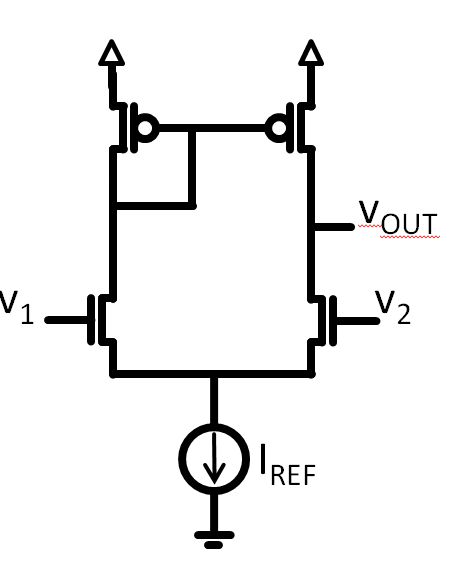
\includegraphics[width=5cm]{figures/fig11-1.png}
    \caption{Exercice 1}
    \label{fig11-1}
\end{figure}

\begin{enumerate}
    \item  Pour $I_{ref}= \SI{10}{\micro A}$, calculez la dynamique de sortie de la paire, la transconductance des transistors d'entrée et la conductance d'Early des 4 transistors.
    \item  Calculez la résistance de sortie de la paire différentielle
    \item  Obtenez l'expression et la valeur du gain en tension de la paire par le principe de superposions.
    \item  Reproduisez les résultats de a, b et c pour $I_{ref}= \SI{100}{\micro A}$.
\end{enumerate}

\hspace{1cm}\hrule\hspace{1cm}

\subsection*{Analyse DC}

Dans cette partie, on néglige l'effet Early. Le circuit est donc symétrique (les PMOS sont identiques et en miroir de courant, les NMOS sont identiques et leur polarisation est identique).
On a donc $I_1 = I_2 = I_{ref}/2$ ($I_1$ et $I_2$ sont les courants dans les branches de gauche et de droite, respectivement).

Soit $V_0$ la tension aux sources des NMOS, on a
\[I_1 = \frac{k_n}{2}\left(V_1-V_0-V_T\right)^2,\]
donc
\[V_0 = -\sqrt{\frac{I_{ref}}{k_n}} = \SI{-0.22}{V}.\]

\paragraph{Dynamique de sortie}$V_{OUT}$ doit être telle que les transistors restent
en régime saturé. Pour le NM0S: $V_{OUT} \ge V_2 - V_T = \SI{0}{V}$.

Pour le PMOS: on calcule la tension de grille des PMOS:
\[I_1 = \frac{k_p}{2}\left(V_{DD}-V_{G,P}-V_T\right)^2,\]
donc $V_{G,P} = \SI{3.78}{V}$.
On a donc $V_{OUT} \le V_{G,P}+V_T = \SI{4.78}{V}$.

\paragraph{Transconductance des transistors d'entrée}
\[g_m = g_{m,1} = g_{m,2} = \frac{2I_1}{-V_0} = \SI{44.7}{\micro S}\]

\paragraph{Conductance d'Early}
\[g_{d,1} = g_{d,2} = g_{d,3} = g_{d,4} = \frac{I_1}{V_A} = \SI{100}{nS}\]

\subsection*{Résistance de sortie}
Schéma petit-signal:
\begin{center}
\begin{circuitikz}
    \draw
    (1, 4) to[short] (-2, 4) to[R=$1/g_{m,3}$, i=$i_3$] (-2, 2) to[cI=$g_{m}v_1$] (-2, 0)
    to[short] (4, 0)
    to[R=$r_0$] (4, 2) to[R=$r_0$] (4, 4) to[short] (1, 4)
    to[cI=$i_3$] (1, 2) to[cI=$g_{m}v_2$] (1, 0)
    (1, 2) to[short, -*] (4, 2) to[short, -o] (5, 2) node[anchor=west] {$v_{out}$}
    (1, 0) node[ground] {}
    (1, 4) node[ground, yscale=-1] {};
\end{circuitikz}
\end{center}
On néglige l'effet Early du transistor 1. En effet, la tension à son drain est
pratiquement constante (vu que le courant dans le transistor 3 varie peu).
De plus, on approxime la conductance du transistor 3 par $g_m$.

On oberve alors que la résistance de sortie est $r_0/2$.

\subsection*{Gain différentiel}
En considérant $v_1 = -v_2 = v_{id}/2$, on applique le principe de superposition:
on applique d'abord $v_1$ et on met $v_2$ à zéro:
\begin{center}
\begin{circuitikz}
    \draw
    (1, 4) to[short] (-2, 4) to[R=$1/g_{m,3}$, i=$i_3$] (-2, 2) to[cI=$g_{m}v_1$] (-2, 0)
    to[short] (4, 0)
    to[R=$r_0$] (4, 2) to[R=$r_0$] (4, 4) to[short] (1, 4)
    to[cI=$i_3$] (1, 2)
    (1, 2) to[short, -*] (4, 2) to[short, -o] (5, 2) node[anchor=west] {$v_{out}$}
    (1, 0) node[ground] {}
    (1, 4) node[ground, yscale=-1] {};
\end{circuitikz}
\end{center}
On a alors un courant $i_3 = g_m v_1$ qui passe dans la
résistance de sortie pour donner une tension $r_0/2 g_m v_1$.

On applique ensuite $v_2$ et on met $v_1$ à zéro:
\begin{center}
\begin{circuitikz}
    \draw
    (1, 4) to[short] (-2, 4) to[R=$1/g_{m,3}$, i=$i_3$] (-2, 2) to[open] (-2, 0)
    to[short] (4, 0)
    to[R=$r_0$] (4, 2) to[R=$r_0$] (4, 4) to[short] (1, 4)
    to[cI=$i_3$] (1, 2) to[cI=$g_{m}v_2$] (1, 0)
    (1, 2) to[short, -*] (4, 2) to[short, -o] (5, 2) node[anchor=west] {$v_{out}$}
    (1, 0) node[ground] {}
    (1, 4) node[ground, yscale=-1] {};
\end{circuitikz}
\end{center}
On a alors un courant $-g_m v_2$ qui passe dans la résistance
de sortie pour donner une tension $-r_0/2 g_m v_2$.

On a donc au total: $v_{out} = r_0/2 g_m (v_1 - v_2) = r_0/2 g_m v_{id}$.
Le gain est alors $A = r_0 g_m / 2 = 224$.

\section*{Exercice 2 : Paire différentielle complexe}

On considère la paire différentielle complexe de la Figure \ref{fig11-2} dans une technologie canal long 1?$\mu$m. Les paramètres technologiques sont dans la table 9.1 du cours. NMOS : 10/2, PMOS : 20/2. 
Obtenez l'expression analytique ainsi que la valeur du gain ($V_{out,+}-V_{out,-}$)/($V_{in,+}-V_{in,-}$).
\begin{figure}[!htbp]
    \centering
    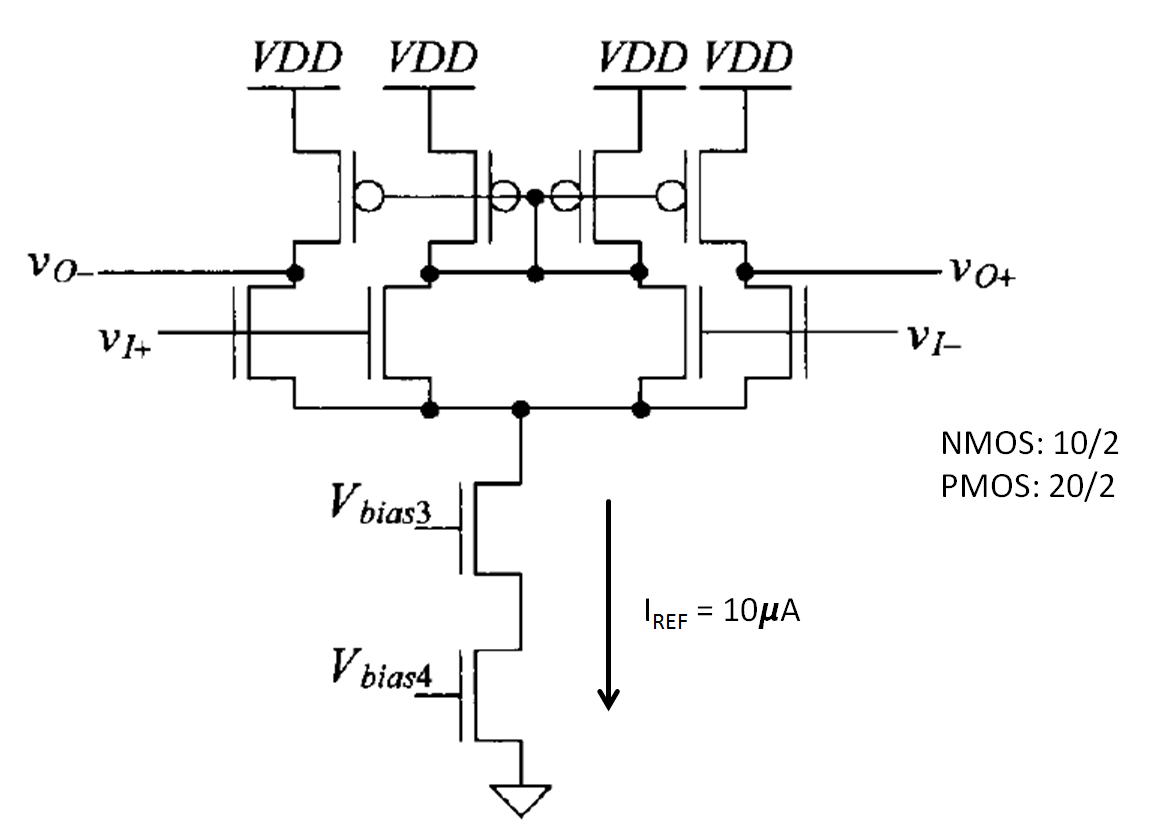
\includegraphics[width=10cm]{figures/fig11-2.png}
    \caption{Exercice 1}
    \label{fig11-2}
\end{figure}

\hspace{1cm}\hrule\hspace{1cm}

Schéma petit-signal:
\begin{center}
    \begin{circuitikz}
        \draw
        (0, 4) node[ground, yscale=-1] {}
        to[R=$1/(2g_m)$, i=$i_0$] (0, 2) to[R=$r_0/2$] (0, 0) node[ground] {}
        (0, 2) -- (2, 2) to[cI=$g_m v_2$] (2, 0) -- (0, 0)
        (0, 2) -- (-2, 2) to[cI=$g_m v_1$] (-2, 0) -- (0, 0)
        (0, 4) -- (4.5, 4) to[cI=$i_0/2$] (4.5, 2) to[cI=$g_m v_2$] (4.5, 0) -- (2, 0)
        (0, 4) -- (-4.5, 4) to[cI=$i_0/2$] (-4.5, 2) to[cI=$g_m v_1$] (-4.5, 0) -- (2, 0)
        (4.5, 4) -- (7, 4) to[R=$r_0$] (7, 2) -- (4.5, 2)
        (-4.5, 4) -- (-7, 4) to[R=$r_0$] (-7, 2) -- (-4.5, 2)
        (7, 2) to[R=$r_0$] (7, 0) -- (4.5, 0)
        (-7, 2) to[R=$r_0$] (-7, 0) -- (-4.5, 0)
        (7, 2) to[-o] (7.5, 2) node[anchor=west] {$v_O+$}
        (-7, 2) to[-o] (-7.5, 2) node[anchor=east] {$v_O-$}
        ;
    \end{circuitikz}
\end{center}

On applique le principe de superposition: on met $v_2 = \SI{0}{V}$.
On a alors (diviseur de courant)
\[i_0 = \frac{2g_m}{2g_m + 2/r_0}g_m v_1.\]
La tension en sortie est donc
\[v_O+ = 0;\]
\[v_O- = \frac{r_0}{2}\left(\frac{i_0}{2} - g_m v_1\right)
= \frac{r_0}{2}\left(\frac{1}{2}\frac{g_m}{g_m+1/r_0} - 1\right)g_m v_1.\]

On calcule ensuite la tension de sortie avec $v_1 = \SI{0}{V}$ (le calcul est identique):
\[v_O+ = \frac{r_0}{2}\left(\frac{1}{2}\frac{g_m}{g_m+1/r_0} - 1\right)g_m v_2;\]
\[v_O- = 0.\]

Il s'ensuit que
\[v_O+ - v_O- = \frac{r_0}{2}\left(\frac{1}{2}\frac{g_m}{g_m+1/r_0}-1\right)g_m(v_1-v_2),\]
le gain différentiel est alors
\[A_{diff} =
\frac{v_O+ - v_O-}{v_1-v_2} = \frac{r_0}{2}\left(\frac{1}{2}\frac{g_m}{g_m+1/r_0}-1\right)g_m.\]

\paragraph{Remarque} $A_{diff}$ est positif, donc $v_1$ est logiquement nommée $v_{in+}$ et
$v_2$, $v_{in-}$.



\end{document}

